\section{ Gantt's diagram}
For this project we had to arrange several deliverables, each one with a strict deadline.
In particular:
\begin{enumerate}
\item RASD - 06/11/2015
\item DD - 04/12/2015
\item INSPECTION - 05/01/2016
\item INTEGRATION TESTING - 21/01/2016
\item PROJECT PLANNING - 02/02/2016
\end{enumerate}

To accomplish the work we folllowed the instructions of each assignment, referring 
to course material and past years projects.
Our team strategy was definying  all together the main guidelines of the document to be created, with one 
scribe. Then at home each of us expanded and clarified the content previously decided.
A special case was the inspection document, when we associated randomly the points in the checklist to each member.

\begin{center}
\begin{figure} [h]

\noindent\makebox[\textwidth]{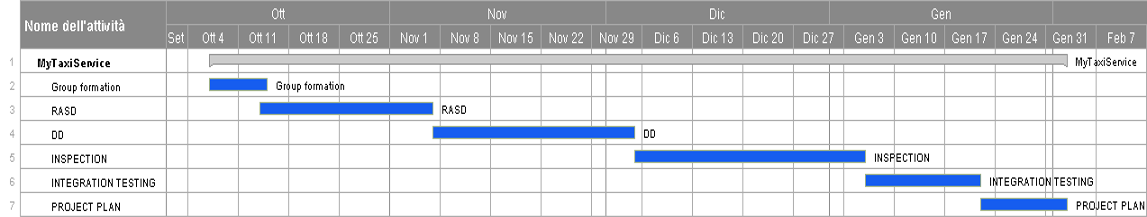
\includegraphics[scale=0.4]{chapters/SWE2-4.png}}

\caption{Gantt's diagram}
 \end{figure}
\end{center}
